\documentclass{protokol}

\usepackage[czech]{babel}
\usepackage[utf8]{inputenc}
\usepackage{icomma}

% Plovouci bloky (obrazky, tabulky)
\usepackage{floatrow}
\floatsetup[table]{capposition=top}
\floatsetup[figure]{frameset={\fboxsep16pt}}
\usepackage{subcaption}

% Tabulky
\usepackage{tabu}
\usepackage{booktabs}
\usepackage{csvsimple}
\usepackage{multirow}
\usepackage{multicol}

% Jednotky
\usepackage{siunitx}
\sisetup{
	locale               = DE,
	inter-unit-product   = \ensuremath{{}\cdot{}},
	list-units           = single,
	list-separator       = {; },
	list-final-separator = \text{ a },
	list-pair-separator  = \text{ a },
	range-phrase         = \text{ až },
	range-units          = single,
}
\usepackage{amsmath}

% Obvody
\usepackage{circuitikz}

% Obrazky a grafy
% \usepackage{graphicx}
\graphicspath{
	{plots/}
	{build/plots/}
	{img/}
}
\usepackage{epstopdf}
\epstopdfsetup{outdir=./build/plots/}

\jmenopraktika={Experimentální metody}
\jmeno={Radek Horňák, Jan Slaný, Lukáš Vrána}
\obor={Fyzika plazmatu}
\skupina={Pá 8:00}
\rocnik={IV}
\semestr={VIII}

\cisloulohy={}
\jmenoulohy={Měření povrchové energie}

\datum={17. května 2022}
\tlak={}% [hPa]
\teplota={}% [C]
\vlhkost={}% [%]

\begin{document}
\header
\section{Úvod}

\section{Praktická část}
\par Pro měření povrchové energie byl použit přístroj See System, viz 
obr.~\ref{ss}. Přístroj je složen ze stolku o~velikosti $10 \times 10$~cm, 
který lze dvěma stavěcími šrouby posouvat do všech směrů, a 2Mpix kamery, která 
snímá povrch. Na stolek se položí substrát, jehož povrchovou energii chceme 
zkoumat. Mikropipetou se nanese na povrch kapka a stolek se stavěcími šrouby 
naladí tak, aby kamera ostře snímala kapku na povrchu. Přístroj je připojen USB 
portem k~počítači, který pomocí příslušného softwaru dokáže ovládat kameru. 
Jakmile je kapka ostře vidět, přes software uložíme fotku z~kamery a dále 
zpracujeme. Na kapce zvolíme ručně tři body -- dvě na rozhraní pevná látka -- 
kapalina -- plyn a třetí bod na vrcholu kapky, čímž určíme kontaktní úhel pro 
danou testovací kapalinu, viz obr.~\ref{ssw}. Pokud toto uděláme pro kapky 
alespoň dvou různých kapalin, software dokáže spočítat povrchovou energii.

\par Měřili jsme povrchovou energii teflonu. Před měřením jsme povrch očistili 
isopropylalkoholem. Následně jsme měřili kontaktní úhel šesti testovacích 
kapalin: voda, ethylenglykol, dijodomethan, glycerol, formamid, 
$\alpha$-bromnaftalen, kde u každé kapaliny jsme naměřili kontaktní úhel 10 
kapek. Pro výpočet povrchové energie jsme použili několik 
modelů.

\begin{figure}
	\begin{center}
		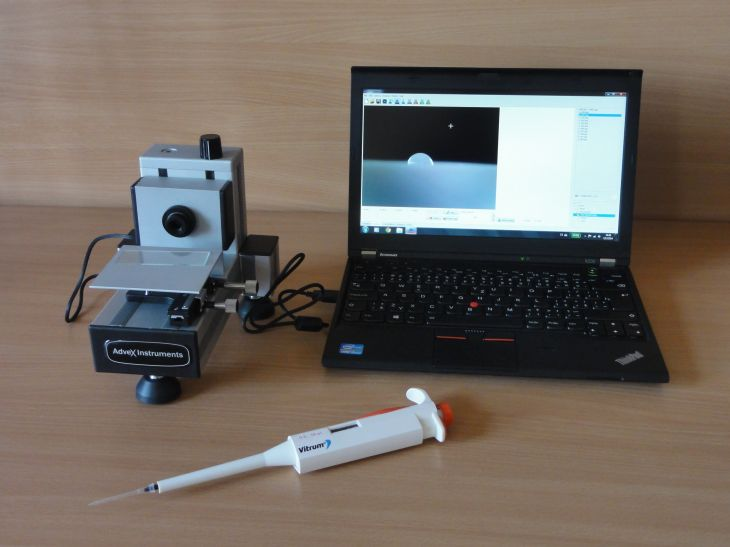
\includegraphics[width=\textwidth]{seesystem.jpg}
		\captionof{figure}{Přístroj See System pro měření kontaktního úhlu 
		kapky a určení povrchové energie.}
		\label{ss}
	\end{center} 
\end{figure}

\begin{figure}
	\begin{center}
		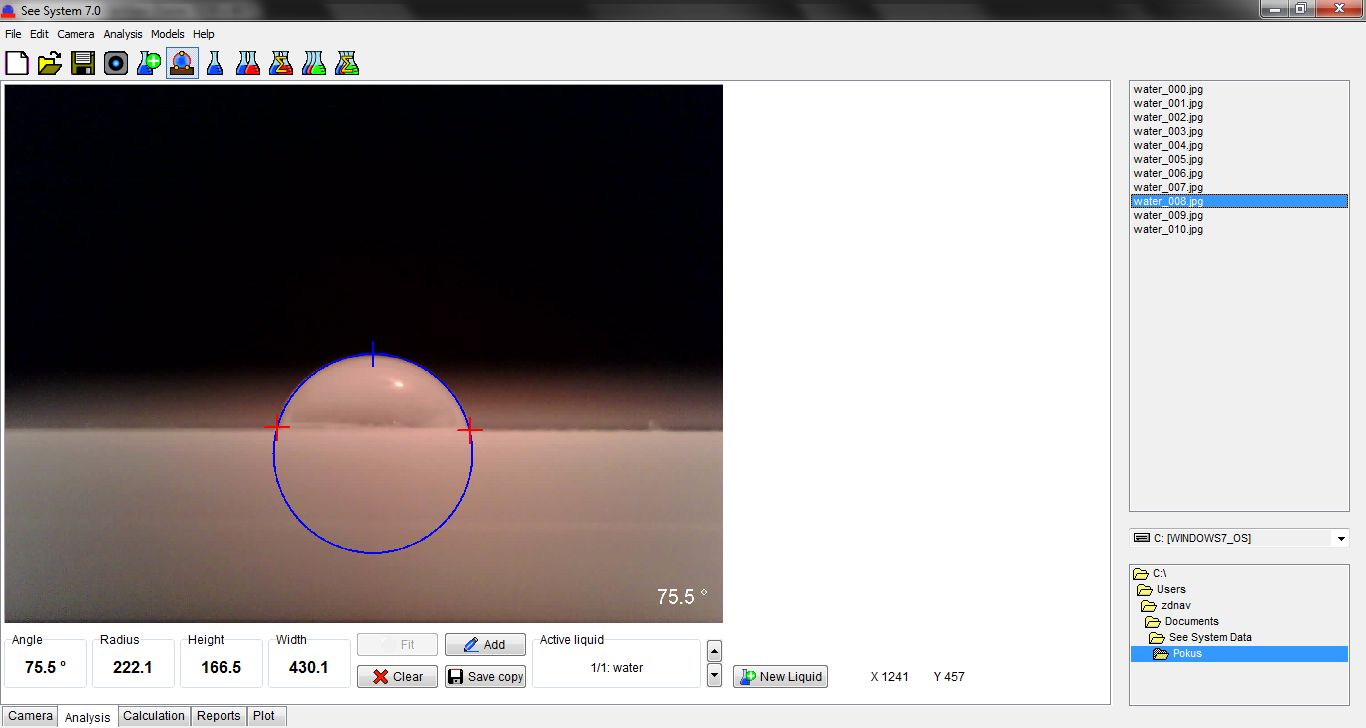
\includegraphics[width=\textwidth]{seesystemsw.jpg}
		\captionof{figure}{Ukázka tříbodového určení kontaktního úhlu pomocí 
		See System softwaru.}
		\label{ssw}
	\end{center} 
\end{figure}

\subsection{Zismanova metoda}
\begin{equation}
	\cos\theta \cong -1 + 
	2\Phi \left( \frac{\gamma_{\text{sv}}} {\gamma_{\text{lv}}} \right) ^{1/2}
\end{equation}
\par 

\subsection{Wu metoda}
\begin{equation}
	\left(1+\cos\theta\right)\gamma_{\text{l}} = 
	4\left(\frac{\gamma_{\text{s}}^\text{d}\gamma_{\text{l}}^\text{d}}{\gamma_{\text{s}}^\text{d}
	 + \gamma_{\text{l}}^\text{d}} + 
	\frac{\gamma_{\text{s}}^\text{p}\gamma_{\text{l}}^\text{p}}{\gamma_{\text{s}}^\text{p}
	 + \gamma_{\text{l}}^\text{p}}\right)
\end{equation}
\par 

\subsection{Owens-Wendtova regresní metoda}
\begin{equation}
	\frac{1+\cos\theta}{2}\frac{\gamma_{\text{l}}}{\sqrt{\gamma_{\text{l}}^\text{d}}}
	 = \sqrt{\gamma_{\text{s}}^\text{d}} + \sqrt{\gamma_{\text{s}}^\text{p}} 
	 \sqrt{\frac{\gamma_{\text{l}}^\text{p}}{\gamma_{\text{l}}^\text{d}}}
\end{equation}
\par 

\subsection{Acidobazická metoda}
\begin{equation}
	\gamma = \gamma^{\text{LW}} + \gamma^{\text{AB}}
\end{equation}
\begin{equation}
	\gamma^{\text{AB}} = 2\sqrt{\gamma^+\gamma^-}
\end{equation}
\begin{equation}
		\left(1+\cos\theta\right)\gamma_{\text{l}} = 
		2\left(\sqrt{\gamma_\text{l}^{\text{LW}}\gamma_\text{s}^{\text{LW}}} + 
		\sqrt{\gamma_\text{l}^{\text{+}}\gamma_\text{s}^{\text{-}}} + 
		\sqrt{\gamma_\text{l}^{\text{-}}\gamma_\text{s}^{\text{+}}}\right)
\end{equation}
\par 

\subsection{Kwok-Neumann metoda}
\begin{equation}
	\cos\theta = -1 + 
2 {\left(\frac{\gamma_{\text{sv}}}{\gamma_{\text{lv}}}\right)}^{1/2} 
\left(1-0,0001057(\gamma_{\text{lv}} - \gamma_{\text{sv}})^2\right)
\end{equation}
\par 

\subsection{Li-Neumann metoda}
\begin{equation}
	\cos\theta = -1 + 
	2 {\left( \frac{\gamma_{\text{sv}}} {\gamma_{\text{lv}}} \right)}^{1/2} 
	\e^{-0,0001247(\gamma_{\text{lv}} - \gamma_{\text{sv}})^2}
\end{equation}
\par 





\section{Závěr}


\end{document}
